\documentclass[a4paper,twoside]{article}
\usepackage{epsfig}
\usepackage{subcaption}
\usepackage{calc}
\usepackage{amsfonts}
\usepackage{bbm}
\usepackage{amssymb}
\usepackage{amstext}
\usepackage{amsmath}
\usepackage{amsthm}
\usepackage{multicol}
\usepackage{pslatex}
\usepackage{apalike}
\usepackage[ruled,vlined]{algorithm2e}
\usepackage[bottom]{footmisc}
\usepackage{enumitem}
\usepackage{booktabs}
\usepackage{float}
\usepackage{multirow}
\usepackage{algorithmicx}
%------------------------------------------------------------------------------
% hack for CVPR/ICCV style
\makeatletter
\@namedef{ver@everyshi.sty}{}
\makeatother

%------------------------------------------------------------------------------
% main packages
%\usepackage[dvipsnames,svgnames,x11names]{xcolor}
\usepackage{tikz}
\usetikzlibrary{arrows.meta,shapes,calc,matrix,fit,positioning,backgrounds,decorations.markings,fadings}
\usepackage{pgfplots}
\usepackage{pgfplotstable}
\usepgfplotslibrary{dateplot}
\pgfplotsset{compat=1.9}
\usepackage{xstring}

%------------------------------------------------------------------------------
% externalization: requires defining \finalcopy first

\usepgfplotslibrary{external}
% \tikzexternalize[prefix=fig/extern/]
\newcommand{\extfig}[2]{\tikzsetnextfilename{#1}{#2}}
\newcommand{\noextfig}[1]{\tikzset{external/export next={false}}{#1}}
\newcommand{\extdata}[1]{\input{#1}}
\IfBeginWith*{\jobname}{fig/extern/}{\finalcopy}{}

%-----------------------------------------------------------------------------
% tikz styles

\tikzstyle{every picture}+=[
	remember picture,
	every text node part/.style={align=center},
	every matrix/.append style={ampersand replacement=\&},
]
\tikzstyle{tight} = [inner sep=0pt,outer sep=0pt]
\tikzstyle{node}  = [draw,circle,tight,minimum size=12pt,anchor=center]
\tikzstyle{op}    = [draw,circle,tight]
\tikzstyle{dot}   = [fill,draw,circle,inner sep=1pt,outer sep=0]
\tikzstyle{pt}    = [fill,draw,circle,inner sep=1.5pt,outer sep=.2pt]
\tikzstyle{box}   = [draw,rectangle,inner sep=3pt]
\tikzstyle{high}  = [black!60]
\tikzstyle{group} = [high,box,opacity=.5]
\tikzstyle{dim1}  = [fill opacity=.3,text opacity=1]
\tikzstyle{dim2}  = [fill opacity=.5,text opacity=1]
\tikzstyle{dim3}  = [fill opacity=.7,text opacity=1]
\tikzstyle{rectc} = [tight,transform shape]
\tikzstyle{rect}  = [rectc,anchor=south west]

%-----------------------------------------------------------------------------
% framed figures

\newcommand{\framed}[3][1]{\extfig{#2}{\tikz{
	\node[tight](a){\fig[#1]{#3}};
	\node[tight,draw=gray,fit=(a)]{};
}}}

%-----------------------------------------------------------------------------
% pgfplots general options

\newcommand{\leg}[1]{\addlegendentry{#1}}

\tikzset{every mark/.append style={solid}}
\pgfplotsset{%smooth,
	grid=both, width=\columnwidth, try min ticks=5,
	every axis/.append style={font=\small},
	every axis plot/.append style={thick,mark=none,mark size=1.8,tension=0.18},
	legend cell align=left, legend style={fill opacity=0.8},
	xticklabel={\pgfmathprintnumber[assume math mode=true]{\tick}},
	yticklabel={\pgfmathprintnumber[assume math mode=true]{\tick}},
	nodes near coords math/.style={
	nodes near coords={\pgfmathprintnumber[assume math mode=true]{\pgfplotspointmeta}},
	},
}

\pgfplotsset{
	dash/.style={mark=o,dashed,opacity=0.6},
	dott/.style={mark=o,dotted,opacity=0.6},
	nolim/.style={enlargelimits=false},
	plain/.style={every axis plot/.append style={},nolim,grid=none},
}
%\pgfplotsset{scaled y ticks = false}
\newcommand{\kilo}[1]{\thisrow{#1}/1000}

%--------------------------------------------------------------------

% layers
\pgfdeclarelayer{bg4}
\pgfdeclarelayer{bg3}
\pgfdeclarelayer{bg2}
\pgfdeclarelayer{bg1}
\pgfdeclarelayer{fg1}
\pgfdeclarelayer{fg2}
\pgfdeclarelayer{fg3}
\pgfdeclarelayer{fg4}
\pgfsetlayers{bg4,bg3,bg2,bg1,main,fg1,fg2,fg3,fg4}

%------------------------------------------------------------------------------
% 3d drawing

\pgfkeys{/tikz/.cd, aspect/.store in=\aspect, aspect=1}
\pgfkeys{/tikz/.cd, depth/.store in=\depth, depth=.5}
\pgfkeys{/tikz/.cd, stepx/.store in=\step, stepx=1}

\tikzstyle{geom} = [line join=bevel,aspect=1,depth=.5,z={(\depth*\aspect,\depth)}]
\tikzstyle{wire} = [geom,draw,thick]

% 3d coordinates
\def\cx[#1,#2,#3]{#1}
\def\cy[#1,#2,#3]{#2}
\def\cz[#1,#2,#3]{#3}
\def\ex[#1,#2,#3]{#1,0,0}
\def\ey[#1,#2,#3]{0,#2,0}
\def\ez[#1,#2,#3]{0,0,#3}

% lines along x, y, or z
\newcommand{\zline}[3][]{%
\path[geom,#1] #2 -- +(\cx[#3],\cy[#3]);
}
\newcommand{\yline}[3][]{%
\path[geom,#1,shift={#2},xslant=\aspect]
	(0,0) -- +(\cx[#3],\depth*\cz[#3]);
}
\newcommand{\xline}[3][]{%
\path[geom,#1,shift={#2},yslant=1/\aspect]
	(0,0) -- +(\aspect*\depth*\cz[#3],\cy[#3]);
}

% rectangles / grids along x, y, or z
\newcommand{\zrect}[3][]{%
\path[geom,#1] #2 rectangle +(\cx[#3],\cy[#3]);
}
\newcommand{\yrect}[3][]{%
\path[geom,#1,shift={#2},xslant=\aspect]
	(0,0) rectangle +(\cx[#3],\depth*\cz[#3]);
}
\newcommand{\xrect}[3][]{%
\path[geom,#1,shift={#2},yslant=1/\aspect]
	(0,0) rectangle +(\aspect*\depth*\cz[#3],\cy[#3]);
}
\newcommand{\xgrid}[3][]{%
\path[geom,#1,shift={#2},yslant=1/\aspect,xstep=\aspect*\depth*\step]
	(0,0) grid +(\aspect*\depth*\cz[#3],\cy[#3]);
}

% parallepiped
\newcommand{\para}[4][]{%
\zrect[#1]{(#3)}{#4}                 % front
\yrect[#1]{($(#3)+(\ey[#4])$)}{#4}   % top
\xrect[#1]{($(#3)+(\ex[#4])$)}{#4}   % right
\path[geom]
	(#3) coordinate(#2-southwest)
	($(#3)+(#4)$) coordinate(#2-northeast)
	($(#3)+(\ey[#4])$) coordinate(#2-northwest)
	($(#3)+(#4)-(\ey[#4])$) coordinate(#2-southeast)
	($(#3)+.5*(\ex[#4])$) coordinate(#2-south)
	($(#3)+(#4)-.5*(\ex[#4])$) coordinate(#2-north)
	($(#3)+.5*(\ex[#4])+.5*(#4)$) coordinate(#2-center)
	(#2-southwest |- #2-center) coordinate(#2-west)
	(#2-center -| #2-northeast) coordinate(#2-east)
	;
}

\floatstyle{plaintop}
\restylefloat{table}


\usepackage{SCITEPRESS}     % Please add other packages that you may need BEFORE the SCITEPRESS.sty package.


\begin{document}

\newcommand{\head}[1]{{\smallskip\noindent\textbf{#1}}}
\newcommand{\alert}[1]{{\color{red}{#1}}}
\newcommand{\sm}{\scriptsize}
\newcommand{\eq}[1]{(\ref{eq:#1})}

\newcommand{\Th}[1]{\textsc{#1}}
\newcommand{\mr}[2]{\multirow{#1}{*}{#2}}
\newcommand{\mc}[2]{\multicolumn{#1}{c}{#2}}
\newcommand{\tb}[1]{\textbf{#1}}
\newcommand{\ch}{\checkmark}

\newcommand{\red}[1]{{\color{red}{#1}}}
\newcommand{\blue}[1]{{\color{blue}{#1}}}
\newcommand{\green}[1]{{\color{green}{#1}}}
\newcommand{\gray}[1]{{\color{gray}{#1}}}

\newcommand{\citeme}[1]{\red{[XX]}}
\newcommand{\refme}[1]{\red{(XX)}}

\newcommand{\fig}[2][1]{\includegraphics[width=#1\linewidth]{fig/#2}}
\newcommand{\figh}[2][1]{\includegraphics[height=#1\linewidth]{fig/#2}}


\newcommand{\tran}{^\top}
\newcommand{\mtran}{^{-\top}}
\newcommand{\zcol}{\mathbf{0}}
\newcommand{\zrow}{\zcol\tran}

\newcommand{\ind}{\mathbbm{1}}
\newcommand{\expect}{\mathbb{E}}
\newcommand{\nat}{\mathbb{N}}
\newcommand{\zahl}{\mathbb{Z}}
\newcommand{\real}{\mathbb{R}}
\newcommand{\proj}{\mathbb{P}}
\newcommand{\prob}{\operatorname{P}}
\newcommand{\normal}{\mathcal{N}}

\newcommand{\mif}{\textrm{if}\ }
\newcommand{\other}{\textrm{otherwise}}
\newcommand{\minimize}{\textrm{minimize}\ }
\newcommand{\maximize}{\textrm{maximize}\ }
\newcommand{\st}{\textrm{subject\ to}\ }

\newcommand{\id}{\operatorname{id}}
\newcommand{\const}{\operatorname{const}}
\newcommand{\sgn}{\operatorname{sgn}}
\newcommand{\var}{\operatorname{Var}}
\newcommand{\mean}{\operatorname{mean}}
\newcommand{\trace}{\operatorname{tr}}
\newcommand{\diag}{\operatorname{diag}}
\newcommand{\vect}{\operatorname{vec}}
\newcommand{\cov}{\operatorname{cov}}
\newcommand{\sign}{\operatorname{sign}}
\newcommand{\prj}{\operatorname{proj}}

\newcommand{\softmax}{\operatorname{softmax}}
\newcommand{\clip}{\operatorname{clip}}

\newcommand{\defn}{\mathrel{:=}}
\newcommand{\peq}{\mathrel{+\!=}}
\newcommand{\meq}{\mathrel{-\!=}}

\newcommand{\floor}[1]{\left\lfloor{#1}\right\rfloor}
\newcommand{\ceil}[1]{\left\lceil{#1}\right\rceil}
\newcommand{\inner}[1]{\left\langle{#1}\right\rangle}
\newcommand{\norm}[1]{\left\|{#1}\right\|}
\newcommand{\abs}[1]{\left|{#1}\right|}
\newcommand{\frob}[1]{\norm{#1}_F}
\newcommand{\card}[1]{\left|{#1}\right|\xspace}

\newcommand{\diff}{\mathrm{d}}
\newcommand{\der}[3][]{\frac{\diff^{#1}#2}{\diff#3^{#1}}}
\newcommand{\ider}[3][]{\diff^{#1}#2/\diff#3^{#1}}
\newcommand{\pder}[3][]{\frac{\partial^{#1}{#2}}{\partial{{#3}^{#1}}}}
\newcommand{\ipder}[3][]{\partial^{#1}{#2}/\partial{#3^{#1}}}
\newcommand{\dder}[3]{\frac{\partial^2{#1}}{\partial{#2}\partial{#3}}}

\newcommand{\wb}[1]{\overline{#1}}
\newcommand{\wt}[1]{\widetilde{#1}}

\def\xssp{\hspace{1pt}}
\def\ssp{\hspace{3pt}}
\def\msp{\hspace{5pt}}
\def\lsp{\hspace{12pt}}

\newcommand{\cA}{\mathcal{A}}
\newcommand{\cB}{\mathcal{B}}
\newcommand{\cC}{\mathcal{C}}
\newcommand{\cD}{\mathcal{D}}
\newcommand{\cE}{\mathcal{E}}
\newcommand{\cF}{\mathcal{F}}
\newcommand{\cG}{\mathcal{G}}
\newcommand{\cH}{\mathcal{H}}
\newcommand{\cI}{\mathcal{I}}
\newcommand{\cJ}{\mathcal{J}}
\newcommand{\cK}{\mathcal{K}}
\newcommand{\cL}{\mathcal{L}}
\newcommand{\cM}{\mathcal{M}}
\newcommand{\cN}{\mathcal{N}}
\newcommand{\cO}{\mathcal{O}}
\newcommand{\cP}{\mathcal{P}}
\newcommand{\cQ}{\mathcal{Q}}
\newcommand{\cR}{\mathcal{R}}
\newcommand{\cS}{\mathcal{S}}
\newcommand{\cT}{\mathcal{T}}
\newcommand{\cU}{\mathcal{U}}
\newcommand{\cV}{\mathcal{V}}
\newcommand{\cW}{\mathcal{W}}
\newcommand{\cX}{\mathcal{X}}
\newcommand{\cY}{\mathcal{Y}}
\newcommand{\cZ}{\mathcal{Z}}

\newcommand{\vA}{\mathbf{A}}
\newcommand{\vB}{\mathbf{B}}
\newcommand{\vC}{\mathbf{C}}
\newcommand{\vD}{\mathbf{D}}
\newcommand{\vE}{\mathbf{E}}
\newcommand{\vF}{\mathbf{F}}
\newcommand{\vG}{\mathbf{G}}
\newcommand{\vH}{\mathbf{H}}
\newcommand{\vI}{\mathbf{I}}
\newcommand{\vJ}{\mathbf{J}}
\newcommand{\vK}{\mathbf{K}}
\newcommand{\vL}{\mathbf{L}}
\newcommand{\vM}{\mathbf{M}}
\newcommand{\vN}{\mathbf{N}}
\newcommand{\vO}{\mathbf{O}}
\newcommand{\vP}{\mathbf{P}}
\newcommand{\vQ}{\mathbf{Q}}
\newcommand{\vR}{\mathbf{R}}
\newcommand{\vS}{\mathbf{S}}
\newcommand{\vT}{\mathbf{T}}
\newcommand{\vU}{\mathbf{U}}
\newcommand{\vV}{\mathbf{V}}
\newcommand{\vW}{\mathbf{W}}
\newcommand{\vX}{\mathbf{X}}
\newcommand{\vY}{\mathbf{Y}}
\newcommand{\vZ}{\mathbf{Z}}

\newcommand{\va}{\mathbf{a}}
\newcommand{\vb}{\mathbf{b}}
\newcommand{\vc}{\mathbf{c}}
\newcommand{\vd}{\mathbf{d}}
\newcommand{\ve}{\mathbf{e}}
\newcommand{\vf}{\mathbf{f}}
\newcommand{\vg}{\mathbf{g}}
\newcommand{\vh}{\mathbf{h}}
\newcommand{\vi}{\mathbf{i}}
\newcommand{\vj}{\mathbf{j}}
\newcommand{\vk}{\mathbf{k}}
\newcommand{\vl}{\mathbf{l}}
\newcommand{\vm}{\mathbf{m}}
\newcommand{\vn}{\mathbf{n}}
\newcommand{\vo}{\mathbf{o}}
\newcommand{\vp}{\mathbf{p}}
\newcommand{\vq}{\mathbf{q}}
\newcommand{\vr}{\mathbf{r}}
\newcommand{\Vs}{\mathbf{s}}
\newcommand{\vt}{\mathbf{t}}
\newcommand{\vu}{\mathbf{u}}
\newcommand{\vv}{\mathbf{v}}
\newcommand{\vw}{\mathbf{w}}
\newcommand{\vx}{\mathbf{x}}
\newcommand{\vy}{\mathbf{y}}
\newcommand{\vz}{\mathbf{z}}

\newcommand{\vone}{\mathbf{1}}
\newcommand{\vzero}{\mathbf{0}}

\newcommand{\valpha}{{\boldsymbol{\alpha}}}
\newcommand{\vbeta}{{\boldsymbol{\beta}}}
\newcommand{\vgamma}{{\boldsymbol{\gamma}}}
\newcommand{\vdelta}{{\boldsymbol{\delta}}}
\newcommand{\vepsilon}{{\boldsymbol{\epsilon}}}
\newcommand{\vzeta}{{\boldsymbol{\zeta}}}
\newcommand{\veta}{{\boldsymbol{\eta}}}
\newcommand{\vtheta}{{\boldsymbol{\theta}}}
\newcommand{\viota}{{\boldsymbol{\iota}}}
\newcommand{\vkappa}{{\boldsymbol{\kappa}}}
\newcommand{\vlambda}{{\boldsymbol{\lambda}}}
\newcommand{\vmu}{{\boldsymbol{\mu}}}
\newcommand{\vnu}{{\boldsymbol{\nu}}}
\newcommand{\vxi}{{\boldsymbol{\xi}}}
\newcommand{\vomikron}{{\boldsymbol{\omikron}}}
\newcommand{\vpi}{{\boldsymbol{\pi}}}
\newcommand{\vrho}{{\boldsymbol{\rho}}}
\newcommand{\vsigma}{{\boldsymbol{\sigma}}}
\newcommand{\vtau}{{\boldsymbol{\tau}}}
\newcommand{\vupsilon}{{\boldsymbol{\upsilon}}}
\newcommand{\vphi}{{\boldsymbol{\phi}}}
\newcommand{\vchi}{{\boldsymbol{\chi}}}
\newcommand{\vpsi}{{\boldsymbol{\psi}}}
\newcommand{\vomega}{{\boldsymbol{\omega}}}

\newcommand{\rLambda}{\mathrm{\Lambda}}
\newcommand{\rSigma}{\mathrm{\Sigma}}

\newcommand{\vLambda}{\bm{\rLambda}}
\newcommand{\vSigma}{\bm{\rSigma}}

\makeatletter
\newcommand*\bdot{\mathpalette\bdot@{.7}}
\newcommand*\bdot@[2]{\mathbin{\vcenter{\hbox{\scalebox{#2}{$\m@th#1\bullet$}}}}}
\makeatother

\makeatletter
\DeclareRobustCommand\onedot{\futurelet\@let@token\@onedot}
\def\@onedot{\ifx\@let@token.\else.\null\fi\xspace}

\def\eg{\emph{e.g}\onedot} \def\Eg{\emph{E.g}\onedot}
\def\ie{\emph{i.e}\onedot} \def\Ie{\emph{I.e}\onedot}
\def\cf{\emph{cf}\onedot} \def\Cf{\emph{Cf}\onedot}
\def\etc{\emph{etc}\onedot} \def\vs{\emph{vs}\onedot}
\def\wrt{w.r.t\onedot} \def\dof{d.o.f\onedot} \def\aka{a.k.a\onedot}
\def\etal{\emph{et al}\onedot}
\makeatother

\newcommand{\relu}{\operatorname{ReLU}}
\newcommand{\gap}{\operatorname{GAP}}
\newcommand{\up}{\operatorname{Up}}
\newcommand{\ce}{\operatorname{CE}}

\newcommand{\cam}{\textrm{CAM}}
\newcommand{\gcam}{\textrm{Grad-CAM}}
\newcommand{\scam}{\textrm{Score-CAM}}

\newcommand{\mae}{\textrm{MAE}}
\newcommand{\mse}{\textrm{MSE}}
\newcommand{\hi}{\textrm{HI}}

\title{A Learning Paradigm for Interpretable Gradients}

%\author{\authorname{Felipe Torres Figueroa\sup{1}\orcidAuthor{0000-0000-0000-0000}, Hanwei Zhang\sup{1}\orcidAuthor{0000-0000-0000-0000} and Third Author Name\sup{2}\orcidAuthor{0000-0000-0000-0000}}

%\author{\authorname{Felipe Torres Figueroa\sup{1}, Hanwei Zhang\sup{1}, Ronan Sicre\sup{1}, Yannis Avrithis\sup{2}\sup{3} and Stephane Ayache\sup{1}}
%\affiliation{\sup{1}Centrale Marseille, Aix Marseille Univ, CNRS, LIS, Marseille, France}
%\affiliation{\sup{2}Athena RC}
%\affiliation{\sup{3}Institute of Advanced Research on Artificial Intelligence (IARAI)}
%\email{\{felipe.torres, hanwei.zhang, ronan.sicre, stephane.ayache\}@lis-lab.fr, yannis@avrithis.net}
%}
%\author{\authorname{Authors}\affiliation{Affiliations}\email{email}}

\keywords{Gradient, Class Activation Maps, Interpretability}

\abstract{This paper studies deep neural networks interpretability and more specifically the production of saliency maps to explain a Convolutional Neural Network (CNN) decision. Most of the existing approaches derive from Class Activation Maps (CAM) and GradCAM. These methods combine information from fully connected layers and gradient through variations of backpropagation. 
We present a novel training approach to improve the gradient of a CNN in terms of interpretability.
In particular, we modify the optimization loss so the gradient obtained from back-propagation at the input image level is similar to the gradient coming from guided backpropagation. The resulting gradient is smoother and offer more interpretable power to the CNN, when applying interpretability methods.}

\onecolumn \maketitle \normalsize \setcounter{footnote}{0} \vfill
%--------------------------------------------------------------------------------------------------
\addchap{Introduction}
%\addcontentsline{toc}{chapter}{Introduction}
\noindent Amongst the sensory information that the brain processes, visual stimuli accounts 
for 90\% of data analyzed \autocite{potter2014detecting}, while consuming a great amount of energy 
in human metabolism (\cite{phelps1981metabolic}). It is argued that a big influence on the 
brain evolution was as a result of improving the capacity to process this kind of data and the 
ensuing  pattern recognition (\cite{mattson2014superior}). 
Currently, these shapes and forms have evolved too: it is no longer common for a human in most 
metropolitan areas, the need to scan the environment for faces that could reveal a potential 
predator; for a change, the patterns that we now seek to unravel also contain products of our own 
imagination: digits and characters, geometrical shapes.\\

\paragraph{Visual Recognition} Understanding the processes behind visual recognition has been a 
prominent research question throughout human history. From the preliminary questionings by greek  
philosphers (\cite{finger2001origins}) to physics based studies like those by Newton and Locke 
(\cite{swenson2010optics}), and more recently with theories like \textit{Unconscious Inference} 
(\cite{gullstrand1909hemholtz}) and \textit{Gestalt} (\cite{wagemans2012century}), many proposals 
to understand and describe this process have been brought forth. Moreover, vision recogniton is not 
only studied in fields like physics, medicine and psychology; 
with the advent of computer science, computational approaches and theories started emerging 
regarding this domain. One such study that proved seminal in this domain is that carried out by 
David Marr (\cite{poggio1981marr}, \cite{marr2010vision}). Most notably, Marr addressed vision on 
three levels: comptational, algorithmic and implementation. In particular, upon the computational 
level, Marr pondered around issues that the visual system answers and their explanation; this 
ultimately led to the formulation of fundamental tasks within computer vision such as object 
recognition and reconstruction. Over the past decade great advancements were made on computer 
vision. In particular with the optimization and popularization of \gls{gpu}, models requiring 
a strong computational power became accesible for researchers. To be specific, the framework 
developed by Yann LeCun (\cite{lecun1998gradient}) got revitalized in 2012 with the introduction of 
AlexNet (\cite{krizhevsky2012imagenet}) where proper leverage of these machines outclassed that of 
more traditional machine learning models, Chapter \ref{ch:rel} discusses this in more depth. 
In this short span of time, several groundbreaking architectures have been proposed, in 
particular the ResNet family (\cite{he2016deep}) has remained relevant given its properties
(\cite{wightman2021resnet}); furthermore, with the introduction of the transformer architecture 
(\cite{vaswani2017attention}) this field of research recieved a new impulse and more powerful 
models based upon its functional unit are being brought forth.\\

\noindent It is not only with the increase of computational power that computer vision has improved over time. 
With the developement, popularization and spread of the internet; large collections of data have been 
formed. These aggregations can be extremely specific for a given end, or 
quite general representing the common interests of its users. Over time, these compilations have 
continued to grow both in volume and variety; still, several curated collections are introduced by 
researchers to experiment and control the development of models such as MNIST (\cite{lecun1998gradient}),
BSDS (\cite{MartinFTM01}), Pascal VOC (\cite{pascal-voc-2012}) and most notably, 
ImageNet (\cite{ILSVRC15}) and MS-COCO (\cite{lin2014microsoft}). Additionally, data collection is
an ongoing and a never ending process; as such, the idea of a dataset containing all types of 
information is no longer deemded a dream but a reality that might come true aided by Big Data in 
the foreseeable future \autocite{chen2014big}.\\

\noindent Taking into consideration the aforementioned  increase on  both compute power and data 
availability, deep learning based models have been steadily adopted and assimiliated within society; 
nowadays its no longer so much a question \textit{whether can a model achieve a given task}, but 
rather a question on \textit{how can this given model perform this task}. Providing an answer to 
this question is paramount as human lives are now being directly affected by such kind of models. 
The main issue behind understanding deep models, lies within the size and complexity of deep 
architecttures, where providing interpretable explanations has lead to the surge of a novel field 
of research (\cite{guidotti2018survey}, \cite{bodria2021benchmarking}).

\paragraph{Interpretability}
To begin discussing about interpretability, one must ponder around its definition. 
Over the last decade, many authors have attempted to address to this question. One 
of the most notable discussions can be found within \emph{The Mythos of Model Interpretability} 
(\cite{mythos_interp}). In this work, Lipton argues that for a model to be interpretable it must 
display two properties, \emph{Transparency} and \emph{Post-Hoc Interpretability}. In one hand, 
\textit{Transparency} answers questions regarding the model structure, training and inference 
processes; while on another hand, \textit{Post-Hoc Interpretability} relates to the explanations 
and information that can be drawn of the model itself.

\noindent Considering these properties, we observe that as machine learning models grew in 
complexity; their transparent properties vanished proportionaly to their size. It can be argued 
that traditional models offer themselves to  transparency due to their straightforward formulation 
and inherent properties. Conversely, in terms of post-hoc interpretations, methods like decision 
trees \cite{breiman2017classification} can be pruned to study their performance by removing 
branches (\cite{lakkaraju2016interpretable},\cite{mothilal2020explaining}). 
On another hand, established techniques such as Principal Component Analysis \gls{pca} 
(\cite{wold1987principal}), can be used to gain insight within data leading to a prediction.\\

\noindent When studying deep models, we find that it is after their size and complexity that their 
interpretable propierties get hindered. Common Convolutional Neural Networks \glspl{cnn} 
rely convolution as their corner stone, coupled with non-linear operations such as 
ReLU (\cite{fukushima1975cognitron}), Sigmoid, and Softmax (\cite{hopfield1985neural}) among others.
This aggregation of convolutions on one hand enables these models to process large quantities of 
data, and to a certain extent generalize; however, it also results in an extensive parameter count,
often reaching of millions, and most recently, even billions (\cite{openai_compute}). The 
computational load required for inference, typically measured in \gls{gflops} further compounds 
complexity.\\

\noindent Among the properties proposed by Lipton, we observe that offering model transparency is a 
rather challenging task. While understanding the behaviour of convolutions and 
self-attention might seem straightforward, it is their aggregation and subsequent flow of information what 
makes this process intricate. Moreover, transparency encompases aspects related to both
inference and training. In this regard, while deep learning research is often seen as an open field;
complete transparency is often disregarded as some authors frequently omit key details in their 
descriptions and methodologies. 

In contrast to transparency, providing post-hoc interpretations from deep models is a 
thriving field, where many of the challenges found within transparency are no longer found.
Within this field, various approaches have been proposed to achieve post-hoc interpretability,
including input masking (\cite{petsiuk2018rise}), attribution generation (\cite{NIPS2017_7062}, 
\cite{zhou2016learning}) and model perturbations 
(\cite{fong2017interpretable}, \cite{fong2019understanding}). Furthermore, the development of 
evaluation methodologies for these approaches has continued in tandem with them 
(\cite{choe2020evaluating}, \cite{chattopadhay2018grad}). Chapter \ref{ch:rel} delves deeper into 
these works. 

\paragraph{Dissertation Outline}
%\addcontentsline{toc}{section}{Dissertation Outline}
\noindent This dissertation is organized in the following manner: In Chapter \ref{ch:rel} we 
introduce a background for image recognition models (Section \ref{rel:sec_imrecon}) and the ensuing 
approaches developed to study the interpretability on them (Section \ref{rel:sec_int}). 
Additionally, we introduce evaluation procedures for these approaches which will be further used to 
evaluate ourproposals.\\

\noindent In Chapter \ref{ch:opticam}, we propose Opti-CAM as a methodology that generates 
optimized saliency maps highlighting the relevant regions on an image towards image classification. 
In Section \ref{sec:av_gain} we extend existing evaluation metrics with a novel measurement for 
model coinfidence. 
In Sections \ref{sec:oc_qual} and \ref{sec:oc_quant} we evaluate the effect of these contributions 
towards interpretability assessment.\\

\noindent Chapter \ref{ch:castream} introduces the Cross Attention Stream, an approach that boosts existing 
architectures interpretable properties. We ste up the modulus of this approach in 
Section \ref{sec:ca_defn} alongside its deployment on Section \ref{sec:ca_design}. 
In Sections \ref{sec:ca_qual} and \ref{sec:ca_quant} we demonstrate the benefits of using this
proposal.\\

\noindent Chapter \ref{ch:grad} characterizes a gradient denoising approach with a gradient denoising 
methodology as an approach to enhance the trainining procedure of current models while improving 
interpretability properties. In Section \ref{sec:grad_defn}, we define the gradient denoising 
protocol alongside the regularization proposals to do so.
Sections \ref{sec:grad_qual} and \ref{sec:grad_quant} illustrate the effects of this paradigmn
in the trained models and its effects on interpretability.\\

\noindent Chapter \ref{ch:zip} raises the Zero-Information algorithm and its usage as a substitute
for mask-dependent evaluation proposals. Section \ref{sec:zip_algo} develops this 
method. Section \ref{sec:zip_insdel} demonstrates its incorporation of this 
algorithm onto evaluation protocols. Section \ref{sec:zip_qual} displays
the effect of this approach when applied to mask patches on images. Section 
\ref{sec:zip_benchmark} displays the results of benchmarking these protocols 
with this approach. \\
    
\noindent Finally, we draw conclusions on our work and detail future research perspectives.
\chapter{Related Work}
\addcontentsline{toc}{chapter}{Related Work}

\section{Image Recognition Models}

\subsection{Convolutional Neural Networks}

\subsection{Attention-Based Architectures}


\section{Interpretability}

\subsection{Transparency}

\subsection{Post-Hoc Interpretability}



%\lipsum[1-2]

\uppercase{\section{Background}}
\label{sec:back}

%This section presents some background information regarding guided back propagation and CAM methods

% (Need to elaborate, talk about stuff in verbatum like Mythos of Model interpretability)\cite{mythos_interp} GuidedBackprop\cite{guidedbackprop} Deconvnet\cite{deconvnet} Perturbation Model\cite{perturb_inter}

\subsection{Guided backpropagation \cite{guidedbackprop}}
The derivative of the $\relu$ unit $v = \relu(u) = [u]_+ = \max(u,0)$ with respect to its input $u$ is $\ider{v}{u} = \ind_{u>0}$. By the chain rule, a signal $\delta v = \ipder{L}{v}$ is then propagated backwards through $\relu$ to $\delta u = \ipder{L}{u}$ as $\delta u = \ind_{u>0} \delta v$, where the partial derivative of any scalar quantity of interest is meant, \eg a loss $L$.

Guided backpropagation \cite{guidedbackprop} changes this to $\delta_G u = \ind_{u>0} \ind_{dv>0} \delta v = \ind_{u>0} [\delta v]_+$, essentially masking out values corresponding to negative entries of both the forward ($u$) and the backward ($\delta v$) signals and thus preventing backward flow of negative gradients.

Considering the partial derivative $\ipder{L}{u}$ of some loss $L$ with respect to a variable $u$, \eg through an entire network or part of it, standard backpropagation with this particular change for $\relu$ units is called \emph{guided backpropagation}. We denote the corresponding guided ``partial derivative'' or \emph{guided gradient} by $\ipder{_G L}{u}$. This backpropagation method allows sharp visualization of high level activations conditioned on input images.

%------------------------------------------------------------------------------

\subsection{CAM-based methods}

CAM-based methods build a saliency map as a linear combination of  activation map. 
Specifically, given a target class $c$ and a set of 2D activation maps $\{A^k\}_{k=1}^K$, % outputed from a convolutional layer of a network, 
CAM \cite{cam} is defined as follows:
%ed by $\relu$
\begin{equation}
	S^c = \relu \left( \sum_{k=1}^K \alpha^c_k A^k \right),
\label{eq:cam}
\end{equation}
where the weight $\alpha^c_k$ determines the contribution of channel $k$ to class $c$. This map $S^c$ and the feature maps $A^k$ are non-negative because both are computed with $\relu$ activation functions. Different CAM-based methods differ primarily in the definition of the weights $\alpha^c_k$.

\paragraph{CAM \cite{cam}}
originally defines $\alpha^c_k$ as the weight connecting channel $k$ to class $c$ in the final classification classifier, assuming $\{A^k\}$ are the feature maps of the last convolutional layer, which is followed by \emph{global average pooling} (GAP) and a single dense layer.

\paragraph{Grad-CAM \cite{gradcam}}

is a generalization of CAM for any networks. If $y^c$ is the logit of class $c$, the weights are obtained by GAP of the partial derivatives of $y^c$ with respect to the feature map $A^k$ of a given layer:
\begin{equation}
    \alpha^c_k = \frac{1}{Z} \sum_{i,j} \pder{y^c}{A^k_{ij}},
\label{eq:gcam}
\end{equation}
where $A^k_{ij}$ denotes the value at spatial location $(i,j)$ of feature map $A^k$ and $Z$ is the total number of spatial locations.

Guided Grad-CAM elementwise-multiplies the saliency maps obtained by Grad-CAM and guided backpropagation, after adjusting spatial resolutions. The resulting visualizations are both class-discriminative (by Grad-CAM) and contain fine-grained detail (by guided backpropagation).

\paragraph{Grad-CAM++ \cite{gradcampp}}

is a generalization of Grad-CAM, where partial derivatives of $y^c$ with respect to $A^k$ are followed by $\relu$ as in guided backpropagation \cite{guidedbackprop} and GAP is replaced by a weighted average:
\begin{equation}
    a^c_k = \sum_{i,j} w^{kc}_{ij} \relu \left( \pder{y^c}{A^k_{ij}} \right).
\label{eq:gcamp}
\end{equation}
The weights $w_{ij}^{kc}$ of the linear combination are
\begin{equation}
    w_{ij}^{kc} = \frac{\pder[2]{y^c}{(A^k_{ij})}}
		{2\pder[2]{y^c}{(A^k_{ij})} + \sum_{a,b} A^k_{ab}\pder[3]{y^c}{(A^k_{ij})}}.
\label{eq:gcampw}
\end{equation}

%\paragraph{Smooth Grad-CAM++ \cite{smoothgradcampp}}

%\green{
%\paragraph{SmoothGrad \cite{smoothgrad}} argues that non-linearities like ReLU activations render derivatives noisy. Thus, to improve smoothness of any derivative $D(x)$ with respect to input image $x$, it takes $m$ Gaussian noise images $\epsilon_i \sim \normal(0,\sigma^2)$ and averages the derivatives with respect to $x + \epsilon_i$:
%\begin{equation}
%    \hat{D}(x) = \frac{1}{m} \sum_{i=1}^m D(x + \epsilon_i).
%\label{eq:smooth}
%\end{equation}
%Smooth Grad-CAM++ \cite{smoothgradcampp} applies this idea to Grad-CAM++ \cite{gradcampp}, essentially replacing all partial derivatives in~\eq{gcamp},\eq{gcampw} by smoothed versions according to~\eq{smooth}.
%}


\paragraph{Score-CAM \cite{scorecam}}

%Following the \emph{increase in confidence} metric proposed in Grad-CAM++, 
computes the weights $a^c_k$ based on the increase in confidence \cite{gradcampp} for class $c$ obtained by masking (element-wise multiplying) the input image $x$ with feature map $A^k$:
\begin{equation}
	a^c_k = f(x \circ s(\up(A^k)))_c - f(x_b)_c,
\label{eq:scam}
\end{equation}
where $\up$ is upsampling to the spatial resolution of $x$, $s$ is linear normalization to range $[0,1]$, $\circ$ is the Hadamard product, $f$ is the classifier mapping of input image to class logits and $x_b$ is a baseline image.

While Score-CAM does not require gradients to compute saliency maps, \eq{scam} requires one forward pass through the network $f$ for each channel $k$ and our method modify filters weights during learning.

\section{Opti-CAM}
\label{sec:opticam}

\subsection{Preliminaries}
\label{sec:prelim}

\paragraph{Notation}
\label{sec:notation}

Consider a classifier network $f: \cX \to \real^C$ that maps an input image $\vx \in \cX$ to a logit vector $\vy = f(\vx) \in \real^C$, where $\cX$ is the image space and $C$ is the number of classes. We denote by $y_c = f(\vx)_c$ the predicted logit and by $p_c = \softmax(\vy)_c \defn e^{y_c} / \sum_j e^{y_j}$ the predicted probability for class $c$. For layer $\ell$ with $K_\ell$ channels, we denote by $A^k_\ell = f^k_\ell(\vx) \in \real^{h_\ell \times w_\ell}$ the feature map for channel $k \in \{1,\dots,K_\ell\}$, with spatial resolution $h_\ell \times w_\ell$. Because of $\relu$ non-linearities, we assume that feature maps are non-negative. Similarly, we denote by $S_\ell \in \real^{h_\ell \times w_\ell}$ a 2D saliency map.

%------------------------------------------------------------------------------

\paragraph{Background: CAM-based saliency maps}
\label{sec:back}

Given a layer $\ell$ and a class of interest $c$, we consider saliency maps given by the general formula
\begin{equation}
	S^c_\ell(\vx) \defn h \left( \sum_k w^c_k A^k_\ell \right),
\label{eq:sal}
\end{equation}
where $w^c_k$ are weights defining a linear combination over channels and $h$ is an activation function. CAM~\citep{zhou2016learning} is defined for the last layer $L$ only with $h$ being the identity mapping and $w^c_k$ being the classifier weight connecting the $k$-th channel with class $c$. Grad-CAM~\citep{selvaraju2017grad} is defined for any layer $\ell$ with $h = \relu$ and weights
\begin{equation}
	w^c_k \defn \gap \left( \pder{y_c}{A^k_\ell} \right),
\label{eq:gcam}
\end{equation}
where $\gap$ is global average pooling.
% and $\softmax(\vy)_c = e^{y_c} / \sum_j e^{y_j}$ is the predicted probability of class $c$.
The motivation for $\relu$ is that we are only interested in features that have a positive effect on the class of interest, \ie pixels whose intensity should be increased in order to increase $y_c$.

Score-CAM~\cite{wang2020score} is also defined for any layer $\ell$ with $h = \relu$ and weights $w^c_k \defn \softmax(\vu^c)_k$.  Softmax normalization considers positive channel contributions only and attends to few feature maps.
%that \alert{produce less highlighted areas in the saliency map}. \iavr{Last part unclear.}
Here, vector $\vu^c \in \real^{K_\ell}$ measures the increase in confidence for class $c$ that compares a known baseline image $\vx_b$ with the input image $\vx$ masked according to feature map $A^k_\ell$, for all channels $k$:
\begin{equation}
	u^c_k \defn f(\vx \odot n(\up(A^k_\ell)))_c - f(\vx_b)_c,
\label{eq:s-cam}
\end{equation}
where $\odot$ is the Hadamard product. For this to work, the feature map $A^k_\ell$ is adapted to $\vx$ first: $\up$ denotes upsampling to the spatial resolution of $\vx$ and
\begin{equation}
	n(A) \defn \frac{A - \min A}{\max A - \min A}
\label{eq:norm}
\end{equation}
\redred{is a normalization of matrix $A$ into $[0,1]$.} While Score-CAM does not need gradients, it requires as many forward passes through the network as the number of channels in the chosen layer, which is computationally expensive.

%------------------------------------------------------------------------------

\paragraph{Motivation}
\label{sec:motiv}

\iavr{Score-CAM considers each feature map as a mask in isolation. How about linear combinations?} Given a vector $\vw \in \real^{K_\ell}$ with $w_k$ its $k$-th element, let
\begin{equation}
	F(\vw) \defn f \left( \vx \odot n \left( \up \left(
		\displaystyle\sum_k w_k A^k_\ell
	\right) \right) \right)_c.
\label{eq:s-obj}
\end{equation}
\ronan{If we assume that $\vx_b = \vzero$ in~\eq{s-cam} and define $n(\vzero) \defn \vzero$ in~\eq{norm}, then we can rewrite the right-hand side of~\eq{s-cam} as
\begin{equation}
	\frac{F(\vw_0 + \delta \ve_k) - F(\vw_0)}{\delta},
\label{eq:s-cam2}
\end{equation}
where $\vw_0 = \vzero$, $\delta = 1$ and $\ve_k$ is the $k$-th standard basis vector of $\real^{K_\ell}$. This resembles the numerical approximation of the derivative $\pder{F}{w_k}(\vw_0)$, except that $\delta$ is not small as usual. One could compute derivatives efficiently by standard backpropagation instead. It is then possible to iteratively optimize $F$ with respect to $\vw$, starting at any $\vw_0$.}

\iavr{As an alternative, consider masking-based methods relying on optimization in the input space, like \emph{meaningful perturbations} (MP)~\cite{fong2017interpretable} or \emph{extremal perturbations}~\citep{fong2019understanding}. In general, optimization takes the form
\begin{equation}
	S^c(\vx) \defn \arg\max_{\vm \in \cM} f(\vx \odot n(\up(\vm)))_c + \lambda R(\vm).
\label{eq:mask}
\end{equation}
Here, a mask $\vm$ is directly optimized and does not rely on feature maps, hence the saliency map $S^x(\vx)$ is not connected to any layer $\ell$. The mask is at the same or lower resolution than the input image. In the latter case, upsampling is still necessary.

In this approach, one indeed computes derivatives by backpropagation and indeed iteratively optimizes $\vm$. However, because $\vm$ is high-dimensional, there are constraints expressed by $\vm \in \cM$, \eg $\vm$ has a certain norm, and regularizers like $R(\vm)$, \eg $\vm$ is smooth in a certain way. This makes optimization harder or more expensive and introduces more hyperparameters like $\lambda$. One could simply constrain $\vm$ to lie in the linear span of $\{A_\ell^k\}_{k=1}^{K_\ell}$ instead, like all CAM-based methods.}

%------------------------------------------------------------------------------

\subsection{Method}
\label{sec:method}

\paragraph{Saliency maps}

As motivated by \autoref{sec:motiv}, we obtain a saliency map as a convex combination of feature maps by optimizing a given objective function with respect to the weights.
In particular, following~\citep{wang2020score}, we use channel weights $w_k \defn \softmax(\vu)_k$, where $\vu \in \real^{K_\ell}$ is a variable.
We then consider saliency map $S_\ell$ in layer $\ell$ as a function of both the input image $\vx$ and variable $\vu$:
\begin{equation}
    S_\ell(\vx; \vu) \defn \sum_k \softmax(\vu)_k A^k_\ell.
\label{eq:v-sal}
\end{equation}
Comparing with~\eq{sal}, $h$ is the identity mapping, because feature maps are non-negative and weights are positive.

%------------------------------------------------------------------------------

\paragraph{Optimization}

Now, given a layer $\ell$ and a class of interest $c$, we find the vector $\vu^*$ that maximizes the classifier confidence for class $c$, when the input image $\vx$ is masked according to saliency map $S_\ell(\vx; \vu^*)$:
\begin{equation}
	\vu^* \defn \arg\max_{\vu} F^c_\ell(\vx; \vu),
\label{eq:opt}
\end{equation}
where we define the objective function
\begin{equation}
	%F^c_\ell(\vx; \vu) \defn \abs{g_c(f(\vx \odot n(\up(S_\ell(\vx; \vu))))) - g_c(f(\vx))}.
	F^c_\ell(\vx; \vu) \defn g_c(f(\vx \odot n(\up(S_\ell(\vx; \vu))))).
\label{eq:obj}
\end{equation}
Here, the saliency map $S_\ell(\vx; \vu)$ is adapted to $\vx$ exactly as in~\eq{s-cam} in terms of resolution and normalization. For \emph{normalization function} $n$, the default is~\eq{norm}. The \emph{selector function} $g_c$ operates on the logit vector $\vy$; the default is to select the logit of class $c$, \ie $g_c(\vy) \defn y_c$. Other choices, including the definition of $F^c_\ell$ itself, are investigated in \autoref{sec:ablation} \redred{and in the supplementary material.}

%------------------------------------------------------------------------------

\paragraph{Opti-CAM}

Putting everything together, we define
\begin{equation}
	S^c_\ell(\vx) \defn S_\ell(\vx; \vu^*) = S_\ell(\vx; \arg\max_{\vu} F^c_\ell(\vx; \vu)),
\label{eq:o-sal}
\end{equation}
where $S_\ell$ and $F^c_\ell$ are defined by~\eq{v-sal} and~\eq{obj} respectively. The objective function $F^c_\ell$~\eq{obj} depends on variable $\vu$ through $S_\ell$~\eq{v-sal}, where the feature maps $A^k_\ell = f^k_\ell(\vx)$ are fixed. Then,~\eq{obj} involves masking and a forward pass through the network $f$, which is also fixed.

\autoref{fig:idea} is an abstract illustration of our method, \iavr{called Opti-CAM}, without details like upsampling and normalization~\eq{obj}. Optimization takes place along the highlighted path from variable $\vu$ to objective function $F^c_\ell$. The saliency map is real-valued and the entire objective function is differentiable in $\vu$. We use Adam optimizer~\citep{kingma2014adam} to solve the optimization problem~\eq{opt}.

%------------------------------------------------------------------------------

\paragraph{Discussion}

By maximizing~\eq{obj}, the saliency map focuses on the regions contributing to class $c$, while masked regions contribute less. This way, the influence of background in the average pooling process is reduced.

The saliency map is expressed as a linear combination of feature maps~\eq{v-sal}, with normalized weights. Hence, the saliency map is discouraged from taking up the entire image, both by the $\softmax$ competition~\eq{v-sal} and by the fact that feature maps only respond to particular locations.

\iavr{In case $g_c(\vy) \defn y_c$,~\eq{o-sal} takes the form of direct masking~\eq{mask} with $R(\vm) = \vzero$ and
\begin{equation}
	\cM \defn \{ S_\ell(\vx; \vu) : \vu \in \real^{K_\ell} \}.
\label{eq:mask-m}
\end{equation}
This constraint makes ours a CAM-based method. It dispenses the need for regularizers, because we only optimize one vector over the feature dimensions\modify{ (up to 2,048 for ResNet50), which is small compared with the dimensions of input images (50k for ImageNet)}. In addition, it does not complicate the optimization process in any way. It is only a different parametrization.}

%------------------------------------------------------------------------------

\iavr{
\section{\AGf ($\AG$)}

\redred{Average drop ($\AD$) and average increase ($\AI$)~\cite{chattopadhay2018grad} are well-established classification metrics. They measure the effect on the predicted class probabilities by masking the input image with the saliency map.} Let $p^c_i$ and $o^c_i$ be the predicted probability for class $c$ given as input the $i$-th test image $\vx_i$ and its masked version respectively. Masking refers to element-wise multiplication with the saliency map, which is at the same resolution as the original image with values in $[0,1]$. Let $N$ be the number of test images. Class $c$ is taken as the ground truth.

\emph{Average drop} ($\AD$) quantifies how much predictive power, measured as class probability, is lost when we only mask the image; lower is better:
\begin{equation}
	\AD(\%) \defn \frac{1}{N} \sum_{i=1}^N \frac{[p^c_i - o^c_i]_+}{p^c_i} \cdot 100.
\label{eq:ad}
\end{equation}

\emph{Average increase} ($\AI$), also known as \emph{increase in confidence}, measures the percentage of images where the masked image yields a higher class probability than the original; higher is better:
\begin{equation}
	\AI(\%) \defn \frac{1}{N} \sum_i^N \ind_{p^c_i < o^c_i} \cdot 100.
\label{eq:ai}
\end{equation}

$\AD$ and $\AI$ are not defined in a symmetric way. $\AD$ measures changes in class probability whereas $\AI$ measures a percentage of images. It is possible that the percentage is high while the actual increase is small. Hence, it is possible that an attribution method improves both. Indeed, \citep{poppi2021revisiting} observes that a trivial method called Fake-CAM outperforms state-of-the-art methods, including Score-CAM, by a large margin. Fake-CAM simply defines a saliency map where the top-left pixel is set to zero and is uniform elsewhere. This questions the purpose of $\AD$ and $\AI$.

Although the authors of~\citep{poppi2021revisiting} make this impressive observation, they use it to motivate the definition of a number of metrics that are orthogonal to the task at hand, \ie measuring the effect of masking to the classifier. By contrast, we address the problem by introducing a new metric to be paired with $\AD$ as a replacement of $\AI$. We define the new metric as follows.

\emph{\Agf} ($\AG$) quantifies how much predictive power, measured as class probability, is gained when we mask the image; higher is better:
\begin{equation}
	\AG(\%) \defn \frac{1}{N} \sum_{i=1}^N \frac{[o^c_i - p^c_i]_+}{1-p^c_i} \cdot 100.
\label{eq:ag}
\end{equation}
This definition is symmetric to the definition of average drop, in the sense that \redred{in absolute value, the numerator in the sum of $\AD, \AG$ is the positive and negative part of $p^c_i - o^c_i$ respectively and the denominator is the maximum value that the numerator can get as a function of $o^c_i$, given that $0 < o^c_i < p^c_i$ and $p^c_i < o^c_i < 1$ respectively.} The two metrics thus compete each other, in the sense that changing $o^c_i$ to improve one leaves the other unchanged or harms it. As we shall see, an extreme example is Fake-CAM, which yields near-perfect $\AD$ but fails completely on $\AG$.
}

\uppercase{\section{Experiments}}

\begin{figure*}[t]
\scriptsize
\centering
\setlength{\tabcolsep}{1.5pt}
\begin{tabular}{cccccccccc}
    {}&\mr{2}{\Th{Input}}&\mc{2}{\Th{Grad-CAM}}&\mc{2}{\Th{Grad-CAM++}}&\mc{2}{\Th{Score-CAM}}&\mc{2}{\Th{Ablation-CAM}}\\
    {}&{}&\Th{Baseline}&\Th{Denoised}&\Th{Baseline}&\Th{Denoised}&\Th{Baseline}&\Th{Denoised}&\Th{Baseline}&\Th{Denoised}\\
  %  {\rotatebox{90}{\small Man}}&
\includegraphics[width=0.09\textwidth]{fig/fig_cam/original/4862.JPEG}&
\includegraphics[width=0.09\textwidth]{fig/fig_cam/baseline/gradcam/4862.JPEG}&
\includegraphics[width=0.09\textwidth]{fig/fig_cam/cosine/gradcam/4862.JPEG}&
\includegraphics[width=0.09\textwidth]{fig/fig_cam/baseline/gradcampp/4862.JPEG}&
\includegraphics[width=0.09\textwidth]{fig/fig_cam/cosine/gradcampp/4862.JPEG}&
\includegraphics[width=0.09\textwidth]{fig/fig_cam/baseline/scorecam/4862.JPEG}&
\includegraphics[width=0.09\textwidth]{fig/fig_cam/cosine/scorecam/4862.JPEG}&
\includegraphics[width=0.09\textwidth]{fig/fig_cam/baseline/ablationcam/4862.JPEG}&
\includegraphics[width=0.09\textwidth]{fig/fig_cam/cosine/ablationcam/4862.JPEG}\\
    
    {\rotatebox{90}{\small Girl}}&
\includegraphics[width=0.09\textwidth]{fig/fig_cam/original/2641.JPEG}&
\includegraphics[width=0.09\textwidth]{fig/fig_cam/baseline/gradcam/2641.JPEG}&
\includegraphics[width=0.09\textwidth]{fig/fig_cam/cosine/gradcam/2641.JPEG}&
\includegraphics[width=0.09\textwidth]{fig/fig_cam/baseline/gradcampp/2641.JPEG}&
\includegraphics[width=0.09\textwidth]{fig/fig_cam/cosine/gradcampp/2641.JPEG}&
\includegraphics[width=0.09\textwidth]{fig/fig_cam/baseline/scorecam/2641.JPEG}&
\includegraphics[width=0.09\textwidth]{fig/fig_cam/cosine/scorecam/2641.JPEG}&
\includegraphics[width=0.09\textwidth]{fig/fig_cam/baseline/ablationcam/2641.JPEG}&
\includegraphics[width=0.09\textwidth]{fig/fig_cam/cosine/ablationcam/2641.JPEG}\\
    
    {\rotatebox{90}{\small Woman}}&\includegraphics[width=0.09\textwidth]{fig/fig_cam/original/5257.JPEG}&\includegraphics[width=0.09\textwidth]{fig/fig_cam/baseline/gradcam/5257.JPEG}&\includegraphics[width=0.09\textwidth]{fig/fig_cam/cosine/gradcam/5257.JPEG}&\includegraphics[width=0.09\textwidth]{fig/fig_cam/baseline/gradcampp/5257.JPEG}&\includegraphics[width=0.09\textwidth]{fig/fig_cam/cosine/gradcampp/5257.JPEG}&\includegraphics[width=0.09\textwidth]{fig/fig_cam/baseline/scorecam/5257.JPEG}&\includegraphics[width=0.09\textwidth]{fig/fig_cam/cosine/scorecam/5257.JPEG}&\includegraphics[width=0.09\textwidth]{fig/fig_cam/baseline/ablationcam/5257.JPEG}&\includegraphics[width=0.09\textwidth]{fig/fig_cam/cosine/ablationcam/5257.JPEG}\\
        
    {\rotatebox{90}{\small Lobster}}&\includegraphics[width=0.09\textwidth]{fig/fig_cam/original/5160.JPEG}&\includegraphics[width=0.09\textwidth]{fig/fig_cam/baseline/gradcam/5160.JPEG}&\includegraphics[width=0.09\textwidth]{fig/fig_cam/cosine/gradcam/5160.JPEG}&\includegraphics[width=0.09\textwidth]{fig/fig_cam/baseline/gradcampp/5160.JPEG}&\includegraphics[width=0.09\textwidth]{fig/fig_cam/cosine/gradcampp/5160.JPEG}&\includegraphics[width=0.09\textwidth]{fig/fig_cam/baseline/scorecam/5160.JPEG}&\includegraphics[width=0.09\textwidth]{fig/fig_cam/cosine/scorecam/5160.JPEG}&\includegraphics[width=0.09\textwidth]{fig/fig_cam/baseline/ablationcam/5160.JPEG}&\includegraphics[width=0.09\textwidth]{fig/fig_cam/cosine/ablationcam/5160.JPEG}\\
    
    {\rotatebox{90}{\small Couch}}&\includegraphics[width=0.09\textwidth]{fig/fig_cam/original/2043.JPEG}&\includegraphics[width=0.09\textwidth]{fig/fig_cam/baseline/gradcam/2043.JPEG}&\includegraphics[width=0.09\textwidth]{fig/fig_cam/cosine/gradcam/2043.JPEG}&\includegraphics[width=0.09\textwidth]{fig/fig_cam/baseline/gradcampp/2043.JPEG}&\includegraphics[width=0.09\textwidth]{fig/fig_cam/cosine/gradcampp/2043.JPEG}&\includegraphics[width=0.09\textwidth]{fig/fig_cam/baseline/scorecam/2043.JPEG}&\includegraphics[width=0.09\textwidth]{fig/fig_cam/cosine/scorecam/2043.JPEG}&\includegraphics[width=0.09\textwidth]{fig/fig_cam/baseline/ablationcam/2043.JPEG}&\includegraphics[width=0.09\textwidth]{fig/fig_cam/cosine/ablationcam/2043.JPEG}\\
    
    
\end{tabular}
\vspace{3pt}
\caption{Saliency map comparison of several CAM-based methods with standard vs our models training on CIFAR-100 examples.}
\label{fig:salient}
\end{figure*}

This section presents the experimental settings, the definition of our evaluation metrics and results.
%Finally, we present qualitative and quantitative results and an ablation study.\\



\subsection{Experimental Set-up}

In the following sections, we evaluate recognition properties and interpretability capabilities of our approach. Specifically, we generate explanations following popular attribution methods derived from CAM \cite{cam} from the \textbf{pytorch-grad-cam} library from Jacob Gildenblat\footnote{https://github.com/jacobgil/pytorch-grad-cam}.

\paragraph{Dataset}
We train and evaluate our models on CIFAR-100 \cite{krizhevsky2009learning}. This dataset contains 60.000 images of 100 categories, split in 50.000 for training and 10.000 for testing. Each image has a resolution of $32\times32$ pixels. This dataset is chosen because of its ease of usage and prototyping properties. 

\paragraph{Settings}
To obtain competitive performance and ensure the replicability of our method, we follow the methodology found in the repository by weiaicunzai \footnote{https://github.com/weiaicunzai/pytorch-cifar100}. Thus, we train each model following the same training procedure. We perform 200 epochs, with a starting learning rate of $10^{-1}$, a batch-size of 128 images, SGD optimizer and a learning rate policy updating said parameter by division over 5 on epochs 60, 120 and 160.  

\subsection{Faithfulness Evaluation via Image Recognition}
Faithfulness evaluation as proposed in \cite{gradcampp} offers insight about the regions of an image that are considered important for recognition, as highlighted by the saliency map $S^c$. 
Specifically, given a class $c$, an image \textit{I} and a computed saliency map $S^c$ are element-wise multiplied to obtain a masked image $M^c$:

\begin{equation*}
    M^c = S^c\circ I
\end{equation*}

This masked image is similar to the original image on the salient areas and becomes black on the non-salient ones.
To evaluate the saliency maps capability, we forward both the image and the masked version through the network to obtain the prediction scores \textit{$Y_i^c$} and \textit{$O_i^c$} respectively. We then compute the following metrics:

\begin{itemize}
    \item \textbf{Average Drop (AD)} 
    Aims at quantifying how much predictive power is lost when we take into consideration the masked image compared to the original one. Lower is better.
    \begin{equation}
        AD(\%) = \sum_{i=1}^N \frac{max(0,Y_i^c- O_i^c)}{Y_i^c}
    \end{equation}
    \label{Average Drop}
    
    \item \textbf{Average Increase (AI)}
    Unlike Average Drop, Average Increase, also known as Increase of Confidence, measures the percentage of instances of the dataset where the masked image offers a higher score than the original images for a specific class. Higher is better.
    
    \begin{equation}
        AI(\%) = \frac{1}{N} \sum_i^N \mathbbm{1}{(Y_i^c<O_i^c)}*100
    \end{equation}

    \item \textbf{Average Gain (AG)} 
    Most recently introduced in Opti-CAM, %\cite{zhang2023opti}, 
    this metric is designed to be a complement for Average Drop. This measurement is meant to quantify the gain in predictive power attained when the masked image is taken in comparison compared to the original one.
     Higher is better.
    \begin{equation}
        AG(\%) = \sum_{i=1}^N \frac{max(0, O_i^c-Y_i^c)}{Y_i^c}
    \end{equation}
\end{itemize}


\subsection{Causal Metrics for Explanations}
Causality evaluation as proposed in RISE \cite{petsiuk2018rise}, aims at evaluating the effect of masking certain elements of the image and retrieving the change in predictive power for a model with the given changes. Thus, the authors proposed \textbf{Insertion} and \textbf{Deletion}.

\begin{itemize}
	\item \textbf{Average Drop (AD)} 
	Aims at quantifying how much predictive power is lost when we take into consideration the masked image compared to the original one. Lower is better.
	\begin{equation}
	AD(\%) = \sum_{i=1}^N \frac{max(0,Y_i^c- O_i^c)}{Y_i^c}
	\end{equation}
	\label{Average Drop}
	
	\item \textbf{Average Increase (AI)}
	Unlike Average Drop, Average Increase, also known as Increase of Confidence, measures the percentage of instances of the dataset where the masked image offers a higher score than the original images for a specific class. Higher is better.
	
	\begin{equation}
	AI(\%) = \frac{1}{N} \sum_i^N \mathbbm{1}{(Y_i^c<O_i^c)}*100
	\end{equation}
	
	\item \textbf{Average Gain (AG)} 
	Most recently introduced in Opti-CAM, %\cite{zhang2023opti}, 
	this metric is designed to be a complement for Average Drop. This measurement is meant to quantify the gain in predictive power attained when the masked image is taken in comparison compared to the original one.
	Higher is better.
	\begin{equation}
	AG(\%) = \sum_{i=1}^N \frac{max(0, O_i^c-Y_i^c)}{Y_i^c}
	\end{equation}
\end{itemize}


\subsection{Qualitative Experiments}
We visualize the effect of our approach on Figure \ref{fig:salient} and \ref{fig:grads}, which  presents saliency maps, respectively gradient, obtained for the baseline model and the one trained with our approach.
%Conversely, to study the effect of our methodology, on Figure \ref{fig:grads} we demonstrate the differences between the gradients of models trained with our approach and without it.

Regarding saliency maps, we observe the differences brought by our training method that improves interpretability metrics.
The differences are particularly important fro Grad-CAM which directly averages the gradient to weigh feature maps.
Interestingly the differences are smaller on Score-CAM that is not gradient based and only obtains changes from the differences in feature maps.

%that there is some degree of overlapping regarding the higlighted regions for each method, however those differences can be explained in part because of the training procedure performed, given accuracies are different between approaches;

%however, it is important to notice that while accuracy might not always be better, these differences between image parts highlighted lead to gains on interpretable recognition. 
Gradient visualizations show a bit less noise and magnitude with our method.
%On another part, while it has been acknowledged that standard gradients are hard to explain and the information conveyed by them is overall hard to interpret, we observe that our approach indeed leads to less noisy gradients; 
Moreover, the object of interest is better covered by gradient activations. 
%images is presented in a clearer way, thus proving the intended behavior of our training.

\begin{figure}[t]
    \centering
    \setlength{\tabcolsep}{3.5pt}
    \begin{tabular}{cccc}
        {}&\mr{2}{\Th{Input}}&\mc{2}{\Th{Gradient}}\\
        {}&{}&\Th{Baseline}&\Th{Ours}\\
        {\rotatebox{90}{\small Bed}}&\includegraphics[width=0.125\textwidth]{fig/fig_grad/original/5415.JPEG}&\includegraphics[width=0.125\textwidth]{fig/fig_grad/baseline/5415.JPEG}&\includegraphics[width=0.125\textwidth]{fig/fig_grad/cosine/5415.JPEG}\\
        
        {\rotatebox{90}{\small Lamp}}&\includegraphics[width=0.125\textwidth]{fig/fig_grad/original/1766.JPEG}&\includegraphics[width=0.125\textwidth]{fig/fig_grad/baseline/1766.JPEG}&\includegraphics[width=0.125\textwidth]{fig/fig_grad/cosine/1766.JPEG}\\

        {\rotatebox{90}{\small Lawnmower}}&\includegraphics[width=0.125\textwidth]{fig/fig_grad/original/8311.JPEG}&\includegraphics[width=0.125\textwidth]{fig/fig_grad/baseline/8311.JPEG}&\includegraphics[width=0.125\textwidth]{fig/fig_grad/cosine/8311.JPEG}\\

        {\rotatebox{90}{\small Maple Tree}}&\includegraphics[width=0.125\textwidth]{fig/fig_grad/original/1198.JPEG}&\includegraphics[width=0.125\textwidth]{fig/fig_grad/baseline/1198.JPEG}&\includegraphics[width=0.125\textwidth]{fig/fig_grad/cosine/1198.JPEG}\\

        {\rotatebox{90}{\small Sunflower}}&\includegraphics[width=0.125\textwidth]{fig/fig_grad/original/8881.JPEG}&\includegraphics[width=0.125\textwidth]{fig/fig_grad/baseline/8881.JPEG}&\includegraphics[width=0.125\textwidth]{fig/fig_grad/cosine/8881.JPEG}\\
    \end{tabular}
    \caption{Visualization of standard gradient with models trained with standard and our approach.}
    \label{fig:grads}
\end{figure}

\subsection{Quantitative Experiments}
We evaluate the effect of training a given model using our proposed approach with \textit{Faithfulness} and \textit{Causality}. Results are reported in Table \ref{tab:C100_quant}.

As we see, our method offers a consistent improvement in terms of interpretability metrics. Specifically, we obtain improvements on both networks and systematically on five out of six metrics. The improvements are higher for AD, AG, and AI. Insertion gets a smaller but consistent improvement and Deletion is almost always worst with our method, but with a very small difference.
This decrease in performance of Deletion may be due to some limitations of the metrics as reported in previous works.%\cite{zhang2023opti}.

It is intereting to note that improvements on Score-CAM means that our training not only improves gradient for interpretability, but also builds better activation maps.

\begin{table}[t]
\centering
\scriptsize
\setlength{\tabcolsep}{2.5pt}
    \begin{tabular}{lcccccc}\\\toprule
        \mc{7}{\Th{\textbf{Recognition Metrics}}}\\\midrule
        \Th{Model}&\Th{Error}& &\Th{$\lambda$}&\Th{Acc}& &\\\midrule
        \mr{2}{\Th{ResNet-18}}&-& &-&\Th{73.42}& &\\
         &\Th{Cosine}& &$7.5\times10^{-3}$&\Th{72.86}& &\\\midrule
         
        \mr{2}{\Th{MobileNet-V2}}&-& &-&\Th{59.43}&\\
         &\Th{Cosine}&  &$1\times10^{-3}$&\Th{62.36}&\\\midrule
        
        \mc{7}{\Th{\textbf{Interpretable Recognition Metrics}}}\\\midrule    
        \mc{7}{\Th{ResNet-18}}\\\midrule
        \Th{Method}&\Th{Error}&\Th{AD$\downarrow$}&\Th{AG$\uparrow$}&\Th{AI$\uparrow$}&\Th{Ins$\uparrow$}&\Th{Del$\downarrow$}\\\hline
        \mr{2}{\Th{Grad-CAM}}&-&30.16&15.23&29.99&58.47&17.47\\
         &\Th{Cosine}&28.09&16.19&31.53&58.76&17.57\\\hline
        \mr{2}{\Th{Grad-CAM++}}&-&31.40&14.17&28.47&58.61&17.05\\
          &\Th{Cosine}&29.78&15.07&29.60&58.90&17.22\\\hline
        \mr{2}{\Th{Score-CAM}}&-&26.49&18.62&33.84&58.42&18.31\\
          &\Th{Cosine}&24.82&19.49&35.51&59.11&18.34\\\hline
        \mr{2}{\Th{Ablation-CAM}}&-&31.96&14.02&28.33&58.36&17.14\\
         &\Th{Cosine}&29.90&15.03&29.61&58.70&17.37\\\hline
        \mr{2}{\Th{Axiom-CAM}}&-&30.16&15.23&29.98&58.47&17.47\\
          &\Th{Cosine}&28.09&16.20&31.53&58.76&17.57\\\midrule

        \mc{7}{\Th{MobileNet-V2}}\\\midrule
        \Th{Method}&\Th{Error}&\Th{AD$\downarrow$}&\Th{AG$\uparrow$}&\Th{AI$\uparrow$}&\Th{Ins$\uparrow$}&\Th{Del$\downarrow$}\\\hline
        \mr{2}{\Th{Grad-CAM}}&-&44.64&6.57&25.62&44.64&14.34\\
         &\Th{Cosine}&40.89&7.31&27.08&45.57&15.20\\\hline
        \mr{2}{\Th{Grad-CAM++}}&-&45.98&6.12&24.10&44.72&14.76\\
          &\Th{Cosine}&40.76&6.85&26.46&45.51&14.92\\\hline
        \mr{2}{\Th{Score-CAM}}&-&40.55&7.85&28.57&45.62&14.52\\
          &\Th{Cosine}&36.34&9.09&30.50&46.35&14.72\\\hline
        \mr{2}{\Th{Ablation-CAM}}&-&45.15&6.38&25.32&44.62&15.03\\
          &\Th{Cosine}&41.13&7.03&26.10&45.38&15.12\\\hline
        \mr{2}{\Th{Axiom-CAM}}&-&44.65&6.57&25.62&44.64&15.27\\
          &\Th{Cosine}&40.89&7.31&27.08&45.57&15.20\\\bottomrule

    \end{tabular}
    \caption{Experiments with cosine error function on CIFAR-100 with ResNet-18 and MobileNet-V2. Accuracy and interpretability metrics are reported.}
    \label{tab:C100_quant}
\end{table}


\subsection{Ablation Experiments}
We conduct ablation experiments using ResNet18. In these experiments we analyze the different regularization proposals mentioned in Section \ref{sec:method} and the impact of the regularization coefficient.

\paragraph{Regularization proposals} 
To validate our selection of regularization function, we train several models following the same training regime while varying the error function. To evaluate these approaches, we focus solely on Grad-CAM attributions. Results are reported in Table \ref{tab:Regs}


\begin{table}
\centering
\scriptsize
\setlength{\tabcolsep}{3.5pt}
    \begin{tabular}{lcccccc}\\\toprule
    \mc{7}{Regularization Selection}\\\midrule
    \Th{Regularizer}&\Th{Acc}&\Th{AD$\downarrow$}&\Th{AG$\uparrow$}&\Th{AI$\uparrow$}&\Th{Ins$\uparrow$}&\Th{Del$\downarrow$}\\\midrule
    - &73.42&30.16&15.23&29.99&58.47&17.47\\
    Cosine&72,86&\textbf{28.09}&\textbf{16.19}&\textbf{31.53}&58.76&17.57\\
    Histogram &73.88&30.39&14.78&29.38&58.52&17.35\\
    MAE & 73,41& 30,33 & 15,06 &29,61 & 58,13 & 17,95\\
    MSE & 73,86& 29,64 & 15,19 &30,11 & \textbf{59,05} & 18,02\\\bottomrule
    \end{tabular}
    \caption{\textbf{Regularization selection: } Evaluation of the four proposed regularization with ResNet-18 on CIFAR-100.}%}
    \label{tab:Regs}
\end{table}

Following these results, we observe a consistent improvement on most metrics for all regularizer options. 
We note that the accuracy remains stable within half a percent of the original model.
However, we note that most options struggle regarding deletion. 
Cosine Similarity however manages to provide improvements in most metrics, while maintaining deletion performance.
 
\paragraph{Regularization coefficient}
Finally we study the behavior of the regularization coefficient $\lambda$ in \ref{eq:total}. We train multiple models with \textit{Cosine Similarity} and a range of values for $\lambda$, see Table \ref{tab:variation}.

We observe that our method is not very sensible to the regularization coefficient and that the value of $7.5e^{-3}$ offers better performances and is thus selected as the default value for $\lambda$.


\begin{table}
\centering
\scriptsize
\setlength{\tabcolsep}{3.5pt}
    \begin{tabular}{lcccccc}\\\toprule
    \mc{7}{Regularization Selection}\\\midrule
    $\lambda$&\Th{Acc}&\Th{AD$\downarrow$}&\Th{AG$\uparrow$}&\Th{AI$\uparrow$}&\Th{Ins$\uparrow$}&\Th{Del$\downarrow$}\\\midrule
    - &73.42&30.16&15.23&29.99&58.47&17.47\\
    $1\times10^{-3}$ &\textbf{73.71}&29.52&15.17&30.03&59.23&\textbf{17.45}\\
    $2.5\times10^{-3}$ &72.99&30.53&15.82&30.56&59.04&17.96\\
    $5\times10^{-3}$ &72.46&30.10&16.06&30.67&57.47&17.80\\
    $7.5\times10^{-3}$ &72.86&\textbf{28.09}&\textbf{16.20}&\textbf{31.53}&58.76&17.57\\
    $1\times10^{-2}$ &73.28&28.97&15.75&31.16&58.99&17.50\\
    $1\times10^{-1}$ &73.00&28.93&16.13&31.55&\textbf{59.66}&17.95\\
    $1$ &73.30&28.44&16.02&31.31&58.64&17.48\\
    $10$ &73.04&29.28&15.23&30.47&58.74&17.47\\\bottomrule
    \end{tabular}
    \caption{\textbf{Regularization coefficient:} Evaluation of the regularization coefficient $\lambda$, using ResNet-18 with \textit{Cosine Similarity} on CIFAR-100.}%}
    \label{tab:variation}
\end{table}


%--------------------------------------------------------------------------------------------------
\section{Conclusion}
\label{sec:ca_conclusion}
In this chapter we observe that attention-based pooling in transformers is the same as 
forming a class agnostic CAM-based saliency map. This map is used to mask the features before 
global average pooling, much like we mask inputs to confirm that the prediction is due to a certain 
object. This observation establishes that transformers have a built-in CAM-based interpretability 
mechanism and allows us to design a similar mechanism for convolutional networks. Masking in feature 
space is much more efficient than in the input space as it requires only one forward pass, although 
of course it is not equivalent because of interactions within the network.\\

\noindent Although the saliency maps obtained with our \Ours are not very different from those 
obtained with \gap, our approach improves a number of CAM-based interpretability methods on a number 
of convolutional networks according to most interpretability metrics, while preserving classification 
accuracy. By doing so, it also enhances the differences in performance between interpretability methods, 
facilitating their evaluation. Further study may be needed to improve the differentiation of saliency 
maps themselves, to possibly make a class specific representation more competitive and to apply the 
approach to more architectures, including transformers.
\bibliographystyle{apalike}
%\tiny
%\scriptsize
\footnotesize

\bibliography{egbib}


\end{document}

